\chapter{Algorismes d'arbres}

\index{arbre}

Un \key{arbre} és un graf connex i acíclic que consta de $n$
nodes i $n-1$ arestes. Quan eliminem qualsevol aresta d'un arbre el dividim en
dos components connexes, i quan afegim qualsevol aresta a un arbre creem un cicle. A
més, sempre hi ha un camí únic entre dos nodes qualsevol d'un arbre.

Per exemple, l'arbre següent consta de 8 nodes i 7 arestes:
\begin{center}
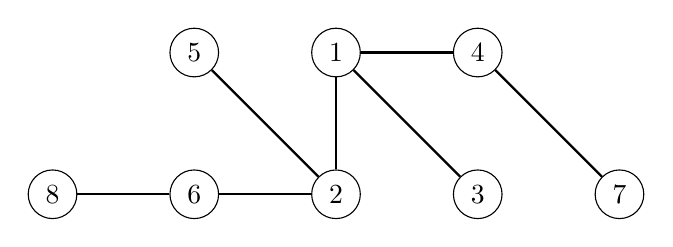
\begin{tikzpicture}[scale=0.9]
\node[draw, circle] (1) at (0,3) {$1$};
\node[draw, circle] (2) at (2,3) {$4$};
\node[draw, circle] (3) at (0,1) {$2$};
\node[draw, circle] (4) at (2,1) {$3$};
\node[draw, circle] (5) at (4,1) {$7$};
\node[draw, circle] (6) at (-2,3) {$5$};
\node[draw, circle] (7) at (-2,1) {$6$};
\node[draw, circle] (8) at (-4,1) {$8$};
\path[draw,thick,-] (1) -- (2);
\path[draw,thick,-] (1) -- (3);
\path[draw,thick,-] (1) -- (4);
\path[draw,thick,-] (2) -- (5);
\path[draw,thick,-] (3) -- (6);
\path[draw,thick,-] (3) -- (7);
\path[draw,thick,-] (7) -- (8);
\end{tikzpicture}
\end{center}


\index{fulla}

Les \key{fulles} d'un arbre són els nodes de grau 1, és a dir, amb
només un veí. Per exemple, les fulles de l'arbre anterior són els
nodes 3, 5, 7 i 8.

\index{arrel} \index{arbre arrelat}

En un arbre \key{arrelat}, un dels nodes s'anomena l'\key{arrel} de
l'arbre, i tots els altres nodes es col·loquen sota l'arrel. Per
exemple, a l'arbre següent, el node 1 és el node arrel.


\begin{center}
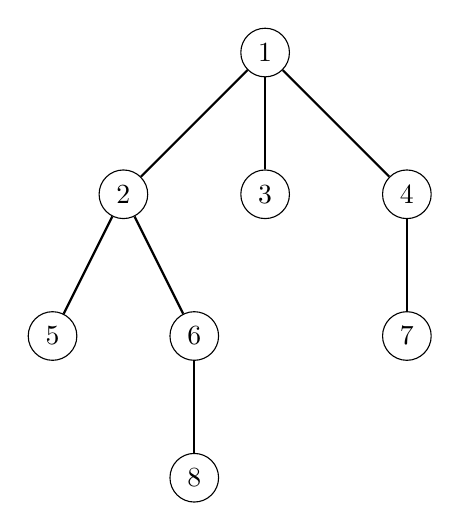
\begin{tikzpicture}[scale=0.9]
\node[draw, circle] (1) at (0,3) {$1$};
\node[draw, circle] (4) at (2,1) {$4$};
\node[draw, circle] (2) at (-2,1) {$2$};
\node[draw, circle] (3) at (0,1) {$3$};
\node[draw, circle] (7) at (2,-1) {$7$};
\node[draw, circle] (5) at (-3,-1) {$5$};
\node[draw, circle] (6) at (-1,-1) {$6$};
\node[draw, circle] (8) at (-1,-3) {$8$};
\path[draw,thick,-] (1) -- (2);
\path[draw,thick,-] (1) -- (3);
\path[draw,thick,-] (1) -- (4);
\path[draw,thick,-] (2) -- (5);
\path[draw,thick,-] (2) -- (6);
\path[draw,thick,-] (4) -- (7);
\path[draw,thick,-] (6) -- (8);
\end{tikzpicture}
\end{center}
\index{fill} \index{pare}

En un arbre arrelat, els \key{fills} d'un node són els seus veïns
inferiors, i el \key{pare} d'un node és el seu veí superior. Cada
node té exactament un pare, excepte l'arrel que no té cap pare. Per
exemple, a l'arbre anterior, els fills del node 2 són els nodes 5 i 6,
i el seu pare és el node 1.

\index{subarbre}

L'estructura d'un arbre arrelat és \emph{recursiva}: cada node de
l'arbre actua com a arrel d'un \key{subarbre} que conté el node en si
i tots els nodes que es troben als subarbres dels seus fills. Per
exemple, a l'arbre anterior, el subarbre del node 2 consta dels nodes
2, 5, 6 i 8:
\begin{center}
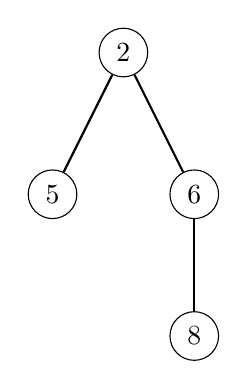
\begin{tikzpicture}[scale=0.9]
\node[draw, circle] (2) at (-2,1) {$2$};
\node[draw, circle] (5) at (-3,-1) {$5$};
\node[draw, circle] (6) at (-1,-1) {$6$};
\node[draw, circle] (8) at (-1,-3) {$8$};
\path[draw,thick,-] (2) -- (5);
\path[draw,thick,-] (2) -- (6);
\path[draw,thick,-] (6) -- (8);
\end{tikzpicture}
\end{center}


\section{Recorregut d'arbres}

Els algorismes generals de recorreguts de grafs es poden utilitzar per
recórrer els nodes d'un arbre. Tanmateix, el recorregut d'un arbre és
més fàcil d'implementar que el d'un graf general, perquè no hi ha
cicles a l'arbre i no és possible arribar a un node des de múltiples
direccions.

La manera típica de recórrer un arbre és iniciar una cerca en
profunditat en un node arbitrari. Es pot fer servir la funció recursiva
següent:


\begin{lstlisting}
void dfs(int s, int e) {
    // process node s
    for (auto u : adj[s]) {
        if (u != e) dfs(u, s);
    }
}
\end{lstlisting}


La funció té dos paràmetres: el node actual $s$ i el node anterior
$e$. El propòsit del paràmetre $e$ és assegurar-se que la cerca només
es mou als nodes que encara no s'han visitat.

El següent codi inicia la cerca al node $x$:


\begin{lstlisting}
dfs(x, 0);
\end{lstlisting}


En la primera crida $e=0$, perquè no hi ha cap node anterior, i es
permet avançar en qualsevol direcció de l'arbre.

\subsubsection{Programació dinàmica}

La programació dinàmica es pot fer servir per calcular informació quan
recorrem un arbre. Per exemple, podem calcular en temps $O(n)$ la mida
del subarbre de cada node, o la longitud del camí més llarg des de
cada node a una fulla.

Com a exemple, calculem per a cada node $s$ un valor
$\texttt{count}[s]$: la mida del seu subarbre. El subarbre conté el
node i tots els nodes dels subarbres dels seus fills, de manera que
podem calcular aquesta mida recursivament amb el codi següent:


\begin{lstlisting}
void dfs(int s, int e) {
    count[s] = 1;
    for (auto u : adj[s]) {
        if (u == e) continue;
        dfs(u, s);
        count[s] += count[u];
    }
}
\end{lstlisting}


\section{Diàmetre}

\index{diàmetre}

El \key{diàmetre} d'un arbre és la longitud màxima d'un camí entre dos
nodes. Per exemple, considereu l'arbre següent:
\begin{center}
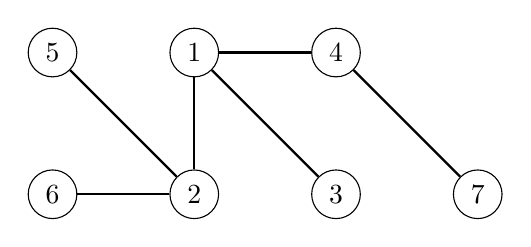
\begin{tikzpicture}[scale=0.9]
\node[draw, circle] (1) at (0,3) {$1$};
\node[draw, circle] (2) at (2,3) {$4$};
\node[draw, circle] (3) at (0,1) {$2$};
\node[draw, circle] (4) at (2,1) {$3$};
\node[draw, circle] (5) at (4,1) {$7$};
\node[draw, circle] (6) at (-2,3) {$5$};
\node[draw, circle] (7) at (-2,1) {$6$};
\path[draw,thick,-] (1) -- (2);
\path[draw,thick,-] (1) -- (3);
\path[draw,thick,-] (1) -- (4);
\path[draw,thick,-] (2) -- (5);
\path[draw,thick,-] (3) -- (6);
\path[draw,thick,-] (3) -- (7);
\end{tikzpicture}
\end{center}
El diàmetre d'aquest arbre és 4, i es correspon al següent camí:
\begin{center}
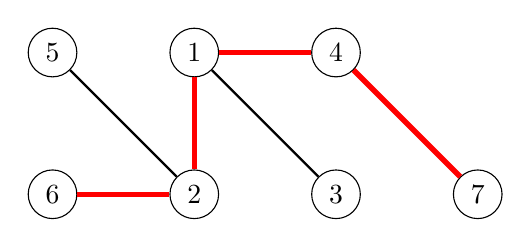
\begin{tikzpicture}[scale=0.9]
\node[draw, circle] (1) at (0,3) {$1$};
\node[draw, circle] (2) at (2,3) {$4$};
\node[draw, circle] (3) at (0,1) {$2$};
\node[draw, circle] (4) at (2,1) {$3$};
\node[draw, circle] (5) at (4,1) {$7$};
\node[draw, circle] (6) at (-2,3) {$5$};
\node[draw, circle] (7) at (-2,1) {$6$};
\path[draw,thick,-] (1) -- (2);
\path[draw,thick,-] (1) -- (3);
\path[draw,thick,-] (1) -- (4);
\path[draw,thick,-] (2) -- (5);
\path[draw,thick,-] (3) -- (6);
\path[draw,thick,-] (3) -- (7);

\path[draw,thick,-,color=red,line width=2pt] (7) -- (3);
\path[draw,thick,-,color=red,line width=2pt] (3) -- (1);
\path[draw,thick,-,color=red,line width=2pt] (1) -- (2);
\path[draw,thick,-,color=red,line width=2pt] (2) -- (5);
\end{tikzpicture}
\end{center}
Tingueu en compte que poden haver-hi diversos camins de longitud
màxima. Al camí anterior, podem substituir el node 6 pel node 5 per
obtenir un altre camí de longitud 4.

A continuació mostrem dos algorismes de temps $O(n)$ que calculen el
diàmetre d'un arbre. El primer algorisme es basa en la programació
dinàmica, i el segon algorisme utilitza dues cerques en profunditat.

\subsubsection{Algorisme 1}

Una manera general d'abordar molts problemes dels arbres és arrelar
primer l'arbre de manera arbitrària. Després d'això, podem intentar
resoldre el problema per separat per a cada subarbre. El nostre primer
algorisme per calcular el diàmetre es basa en aquesta idea.

Una observació important és que cada camí d'un arbre arrelat té un
\emph{punt més alt}: el node més alt que pertany al camí. Així, podem
trobar per a cada node $x$ el camí més llarg que té $x$ com a node més alt
del camí. Un d'aquests camins correspon al diàmetre de l'arbre.

Per exemple, a l'arbre següent, el node 1 és el punt més alt del camí
que correspon al diàmetre:
\begin{center}
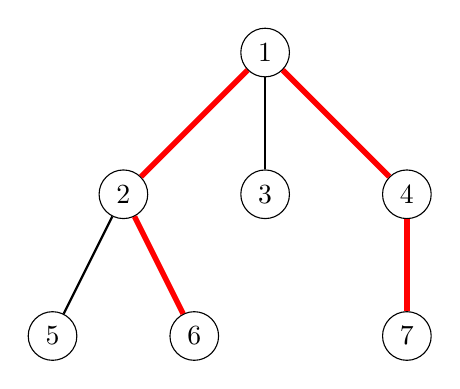
\begin{tikzpicture}[scale=0.9]
\node[draw, circle] (1) at (0,3) {$1$};
\node[draw, circle] (2) at (2,1) {$4$};
\node[draw, circle] (3) at (-2,1) {$2$};
\node[draw, circle] (4) at (0,1) {$3$};
\node[draw, circle] (5) at (2,-1) {$7$};
\node[draw, circle] (6) at (-3,-1) {$5$};
\node[draw, circle] (7) at (-1,-1) {$6$};
\path[draw,thick,-] (1) -- (2);
\path[draw,thick,-] (1) -- (3);
\path[draw,thick,-] (1) -- (4);
\path[draw,thick,-] (2) -- (5);
\path[draw,thick,-] (3) -- (6);
\path[draw,thick,-] (3) -- (7);

\path[draw,thick,-,color=red,line width=2pt] (7) -- (3);
\path[draw,thick,-,color=red,line width=2pt] (3) -- (1);
\path[draw,thick,-,color=red,line width=2pt] (1) -- (2);
\path[draw,thick,-,color=red,line width=2pt] (2) -- (5);
\end{tikzpicture}
\end{center}


Calculem per a cada node $x$ dos valors:
\begin{itemize}
\item $\texttt{toLeaf}(x)$: the maximum length of a path from $x$ to any leaf
\item $\texttt{maxLength}(x)$: the maximum length of a path
whose highest point is $x$
\end{itemize}
Per exemple, a l'arbre anterior, $\texttt{toLeaf}(1)=2$, perquè hi ha
un camí $1 \rightarrow 2 \rightarrow 6$, i $\texttt{maxLength}(1)=4$,
perquè hi ha un camí $6 \rightarrow 2 \rightarrow 1 \rightarrow 4
\rightarrow 7$. En aquest cas, $\texttt{maxLength}(1)$ és igual al
diàmetre.

La programació dinàmica es pot utilitzar per calcular els valors
anteriors per a tots els nodes en temps $O(n)$. Primer, per calcular
$\texttt{toLeaf}(x)$, considerem els fills $c$ de $x$ i afegim un al
màxim dels valors $\texttt{toLeaf}(c)$. A continuació, per a calcular
$\texttt{maxLength}(x)$ escollim dos fills diferents $a$ i $b$ de
manera que la suma $\texttt{toLeaf}(a)+\texttt{toLeaf}(b)$ sigui
màxima, i afegim dos a aquesta suma.

\subsubsection{Algorisme 2}

Una altra manera eficient de calcular el diàmetre d'un arbre es fer
dues cerques en profunditat. Primer, triem un node arbitrari $a$ de
l'arbre i trobem el node $b$ més llunyà de $a$. Aleshores, trobem el
node més llunyà $c$ de $b$. El diàmetre de l'arbre és la distància
entre $b$ i $c$.

Al graf següent, $a$, $b$ i $c$ podrien ser:
\begin{center}
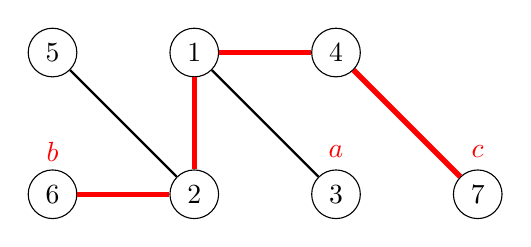
\begin{tikzpicture}[scale=0.9]
\node[draw, circle] (1) at (0,3) {$1$};
\node[draw, circle] (2) at (2,3) {$4$};
\node[draw, circle] (3) at (0,1) {$2$};
\node[draw, circle] (4) at (2,1) {$3$};
\node[draw, circle] (5) at (4,1) {$7$};
\node[draw, circle] (6) at (-2,3) {$5$};
\node[draw, circle] (7) at (-2,1) {$6$};
\path[draw,thick,-] (1) -- (2);
\path[draw,thick,-] (1) -- (3);
\path[draw,thick,-] (1) -- (4);
\path[draw,thick,-] (2) -- (5);
\path[draw,thick,-] (3) -- (6);
\path[draw,thick,-] (3) -- (7);
\node[color=red] at (2,1.6) {$a$};
\node[color=red] at (-2,1.6) {$b$};
\node[color=red] at (4,1.6) {$c$};

\path[draw,thick,-,color=red,line width=2pt] (7) -- (3);
\path[draw,thick,-,color=red,line width=2pt] (3) -- (1);
\path[draw,thick,-,color=red,line width=2pt] (1) -- (2);
\path[draw,thick,-,color=red,line width=2pt] (2) -- (5);
\end{tikzpicture}
\end{center}


Aquest és un mètode elegant, però per què funciona?

És útil dibuixar l'arbre de manera que el camí que
correspon al diàmetre sigui horitzontal i tots els altres nodes en
pengin:
\begin{center}
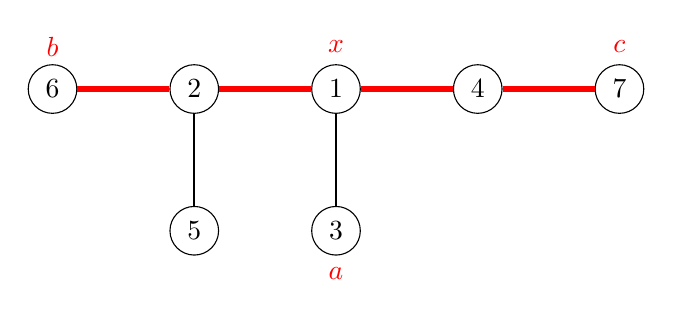
\begin{tikzpicture}[scale=0.9]
\node[draw, circle] (1) at (2,1) {$1$};
\node[draw, circle] (2) at (4,1) {$4$};
\node[draw, circle] (3) at (0,1) {$2$};
\node[draw, circle] (4) at (2,-1) {$3$};
\node[draw, circle] (5) at (6,1) {$7$};
\node[draw, circle] (6) at (0,-1) {$5$};
\node[draw, circle] (7) at (-2,1) {$6$};
\path[draw,thick,-] (1) -- (2);
\path[draw,thick,-] (1) -- (3);
\path[draw,thick,-] (1) -- (4);
\path[draw,thick,-] (2) -- (5);
\path[draw,thick,-] (3) -- (6);
\path[draw,thick,-] (3) -- (7);
\node[color=red] at (2,-1.6) {$a$};
\node[color=red] at (-2,1.6) {$b$};
\node[color=red] at (6,1.6) {$c$};
\node[color=red] at (2,1.6) {$x$};

\path[draw,thick,-,color=red,line width=2pt] (7) -- (3);
\path[draw,thick,-,color=red,line width=2pt] (3) -- (1);
\path[draw,thick,-,color=red,line width=2pt] (1) -- (2);
\path[draw,thick,-,color=red,line width=2pt] (2) -- (5);
\end{tikzpicture}
\end{center}


El node $x$ indica el lloc on el camí des del node $a$ s'uneix al camí
que correspon al diàmetre. El node més allunyat de $a$ és el node $b$,
el node $c$ o algun altre node que estigui almenys tan lluny del node
$x$, i que, per tant, hagués pogut reemplaçar a $b$ o $c$ com a punt
final del camí que es correspon al diàmetre.

\section{Tots els camins més llargs}

El problema següent és calcular per a cada node de l'arbre la longitud
màxima d'un camí que comença al node. Això és una generalització del
problema del diàmetre de l'arbre, perquè la longitud màxima
és el diàmetre de l'arbre. Aquest problema també es pot resoldre en
temps $O(n)$.

Com a exemple, considereu l'arbre següent:
\begin{center}
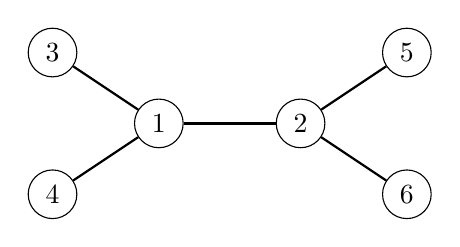
\begin{tikzpicture}[scale=0.9]
\node[draw, circle] (1) at (0,0) {$1$};
\node[draw, circle] (2) at (-1.5,-1) {$4$};
\node[draw, circle] (3) at (2,0) {$2$};
\node[draw, circle] (4) at (-1.5,1) {$3$};
\node[draw, circle] (6) at (3.5,-1) {$6$};
\node[draw, circle] (7) at (3.5,1) {$5$};
\path[draw,thick,-] (1) -- (2);
\path[draw,thick,-] (1) -- (3);
\path[draw,thick,-] (1) -- (4);
\path[draw,thick,-] (3) -- (6);
\path[draw,thick,-] (3) -- (7);
\end{tikzpicture}
\end{center}


Sigui $\texttt{maxLength}(x)$ la longitud màxima d'un camí que comença
al node $x$. Per exemple, a l'arbre anterior,
$\texttt{maxLength}(4)=3$, perquè hi ha un camí $4 \rightarrow 1
\rightarrow 2 \rightarrow 6$. Aquí teniu una taula completa dels
valors:
\begin{center}
\begin{tabular}{l|lllllll}
node $x$ & 1 & 2 & 3 & 4 & 5 & 6 \\
$\texttt{maxLength}(x)$ & 2 & 2 & 3 & 3 & 3 & 3 \\
\end{tabular}
\end{center}


A l'igual que abans, un bon punt de partida per resoldre el problema
és arrelar l'arbre de manera arbitrària:
\begin{center}
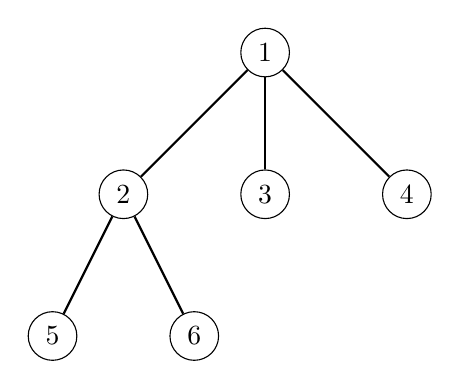
\begin{tikzpicture}[scale=0.9]
\node[draw, circle] (1) at (0,3) {$1$};
\node[draw, circle] (2) at (2,1) {$4$};
\node[draw, circle] (3) at (-2,1) {$2$};
\node[draw, circle] (4) at (0,1) {$3$};
\node[draw, circle] (6) at (-3,-1) {$5$};
\node[draw, circle] (7) at (-1,-1) {$6$};
\path[draw,thick,-] (1) -- (2);
\path[draw,thick,-] (1) -- (3);
\path[draw,thick,-] (1) -- (4);
\path[draw,thick,-] (3) -- (6);
\path[draw,thick,-] (3) -- (7);
\end{tikzpicture}
\end{center}


La primera part del problema és calcular per a cada node $x$ la
longitud màxima d'un camí que passa per un fill de $x$. Per exemple,
el camí més llarg des del node 1 passa pel seu fill 2:
\begin{center}
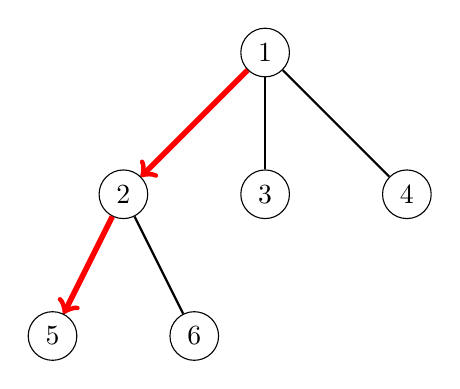
\begin{tikzpicture}[scale=0.9]
\node[draw, circle] (1) at (0,3) {$1$};
\node[draw, circle] (2) at (2,1) {$4$};
\node[draw, circle] (3) at (-2,1) {$2$};
\node[draw, circle] (4) at (0,1) {$3$};
\node[draw, circle] (6) at (-3,-1) {$5$};
\node[draw, circle] (7) at (-1,-1) {$6$};
\path[draw,thick,-] (1) -- (2);
\path[draw,thick,-] (1) -- (3);
\path[draw,thick,-] (1) -- (4);
\path[draw,thick,-] (3) -- (6);
\path[draw,thick,-] (3) -- (7);

\path[draw,thick,->,color=red,line width=2pt] (1) -- (3);
\path[draw,thick,->,color=red,line width=2pt] (3) -- (6);
\end{tikzpicture}
\end{center}
Aquesta part és fàcil de resoldre en temps $O(n)$ fent servir programació dinàmica,
com abans.

La segona part del problema és calcular per a cada node $x$
la longitud màxima d'un camí a través del seu pare $p$. Per exemple,
el camí més llarg des del node 3 passa pel seu pare 1:
\begin{center}
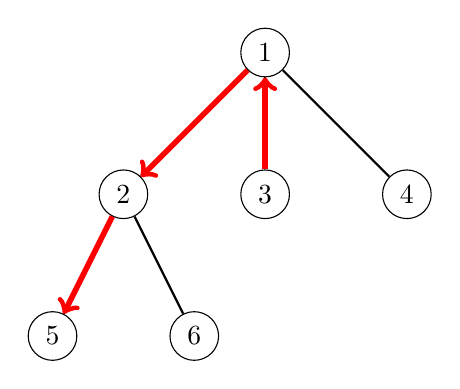
\begin{tikzpicture}[scale=0.9]
\node[draw, circle] (1) at (0,3) {$1$};
\node[draw, circle] (2) at (2,1) {$4$};
\node[draw, circle] (3) at (-2,1) {$2$};
\node[draw, circle] (4) at (0,1) {$3$};
\node[draw, circle] (6) at (-3,-1) {$5$};
\node[draw, circle] (7) at (-1,-1) {$6$};
\path[draw,thick,-] (1) -- (2);
\path[draw,thick,-] (1) -- (3);
\path[draw,thick,-] (1) -- (4);
\path[draw,thick,-] (3) -- (6);
\path[draw,thick,-] (3) -- (7);

\path[draw,thick,->,color=red,line width=2pt] (4) -- (1);
\path[draw,thick,->,color=red,line width=2pt] (1) -- (3);
\path[draw,thick,->,color=red,line width=2pt] (3) -- (6);
\end{tikzpicture}
\end{center}


A primera vista, sembla que hauríem de triar el camí més llarg que surt
de $p$. Tanmateix, això \emph{no} sempre funciona, perquè el camí més
llarg des de $p$ pot passar per $x$. Aquí teniu un exemple d'aquesta
situació:
\begin{center}
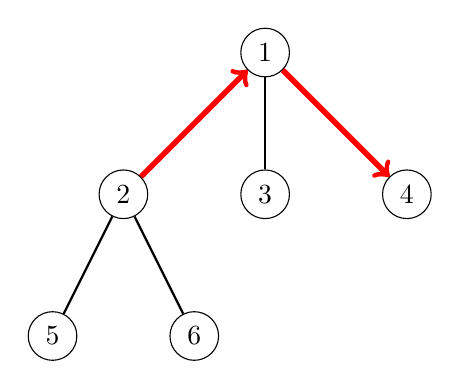
\begin{tikzpicture}[scale=0.9]
\node[draw, circle] (1) at (0,3) {$1$};
\node[draw, circle] (2) at (2,1) {$4$};
\node[draw, circle] (3) at (-2,1) {$2$};
\node[draw, circle] (4) at (0,1) {$3$};
\node[draw, circle] (6) at (-3,-1) {$5$};
\node[draw, circle] (7) at (-1,-1) {$6$};
\path[draw,thick,-] (1) -- (2);
\path[draw,thick,-] (1) -- (3);
\path[draw,thick,-] (1) -- (4);
\path[draw,thick,-] (3) -- (6);
\path[draw,thick,-] (3) -- (7);

\path[draw,thick,->,color=red,line width=2pt] (3) -- (1);
\path[draw,thick,->,color=red,line width=2pt] (1) -- (2);
\end{tikzpicture}
\end{center}


Tot i així, podem resoldre la segona part en temps $O(n)$
emmagatzemant \emph{dues} longituds màximes per a cada node $x$:
\begin{itemize}
\item $\texttt{maxLength}_1(x)$:
the maximum length of a path from $x$
\item $\texttt{maxLength}_2(x)$
the maximum length of a path from $x$
in another direction than the first path
\end{itemize}
Per exemple, al graf anterior, $\texttt{maxLength}_1(1)=2$ utilitzant
el camí $1 \rightarrow 2 \rightarrow 5$, i $\texttt{maxLength}_2(1)=1$
utilitzant el camí $1 \rightarrow 3$.

Finalment, si el camí que correspon a $\texttt{maxLength}_1(p)$ passa
per $x$, arribem a la conclusió que la longitud màxima és
$\texttt{maxLength}_2(p)+1$, i en cas contrari la longitud màxima és
$\texttt{maxLength}_1(p)+1$.



\section{Arbres binaris}

\index{arbre binari}


\begin{samepage}
A \key{binary tree} is a rooted tree
where each node has a left and right subtree.
It is possible that a subtree of a node is empty.
Thus, every node in a binary tree has
zero, one or two children.

For example, the following tree is a binary tree:
\begin{center}
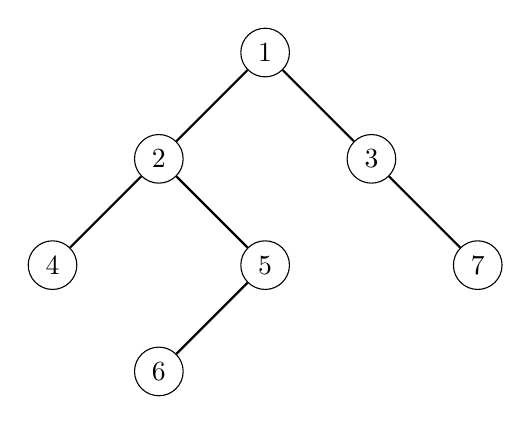
\begin{tikzpicture}[scale=0.9]
\node[draw, circle] (1) at (0,0) {$1$};
\node[draw, circle] (2) at (-1.5,-1.5) {$2$};
\node[draw, circle] (3) at (1.5,-1.5) {$3$};
\node[draw, circle] (4) at (-3,-3) {$4$};
\node[draw, circle] (5) at (0,-3) {$5$};
\node[draw, circle] (6) at (-1.5,-4.5) {$6$};
\node[draw, circle] (7) at (3,-3) {$7$};

\path[draw,thick,-] (1) -- (2);
\path[draw,thick,-] (1) -- (3);
\path[draw,thick,-] (2) -- (4);
\path[draw,thick,-] (2) -- (5);
\path[draw,thick,-] (5) -- (6);
\path[draw,thick,-] (3) -- (7);
\end{tikzpicture}
\end{center}
\end{samepage}


\index{pre-ordre} \index{in-ordre} \index{post-ordre}

Els nodes d'un arbre binari tenen tres ordenacions naturals que es
corresponen a maneres distintes de recórrer l'arbre recursivament:


\begin{itemize}
\item \key{pre-order}: first process the root,
then traverse the left subtree, then traverse the right subtree
\item \key{in-order}: first traverse the left subtree,
then process the root, then traverse the right subtree
\item \key{post-order}: first traverse the left subtree,
then traverse the right subtree, then process the root
\end{itemize}


Per a l'arbre anterior, l'ordenació dels nodes de l'arbre en pre-ordre
és $[1,2,4,5,6,3,7]$, en in-ordre és $[4,2,6,5,1,3,7] $ i en
post-ordre és $[4,6,5,2,7,3,1]$.

Si coneixem l'ordenació en pre-ordre i in-ordre d'un arbre, podem
reconstruir l'estructura exacta de l'arbre. Per exemple, l'arbre
anterior és l'únic arbre possible amb pre-ordre $[1,2,4,5,6,3,7]$ i
in-ordre $[4,2,6,5,1,3, 7]$. De manera similar, si tenim l'ordenació
en post-ordre i in-ordre també podem determinar l'estructura d'un
arbre.

Tanmateix, la situació és diferent si només coneixem l'ordenació en
pre-ordre i post-ordre d'un arbre. En aquest cas, pot haver-hi més
d'un arbre que coincideix amb les ordenacions. Per exemple, els dos
arbres
\begin{center}
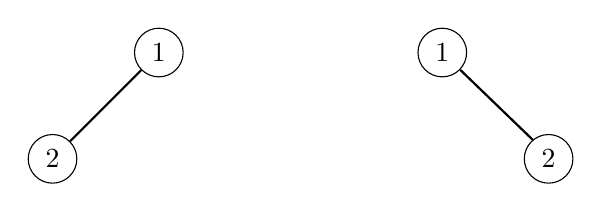
\begin{tikzpicture}[scale=0.9]
\node[draw, circle] (1) at (0,0) {$1$};
\node[draw, circle] (2) at (-1.5,-1.5) {$2$};
\path[draw,thick,-] (1) -- (2);

\node[draw, circle] (1b) at (0+4,0) {$1$};
\node[draw, circle] (2b) at (1.5+4,-1.5) {$2$};
\path[draw,thick,-] (1b) -- (2b);
\end{tikzpicture}
\end{center}
tenen pre-ordre $[1,2]$ i post-ordre $[2,1]$, però les estructures
dels arbres són diferents.



